\subsection{2D Vector Graphics}
Vector graphics is a form of computer graphics where mathematical expressions are used to describe an image.
The image, or the 'scene', is made up of primitives that describe paths, lines and curves, and sometimes combinations of these in order to create more complex shapes.

By relying on mathematical expressions instead of pixel values relative to screen resolution, vector graphics can be described as resolution independent.
This is often conceptualized in the form of scaling:
While scaling a rasterized image will result in a blurry image, scaling a vectorized image will result in the mathematical expressions being recalculated, and the image will remain sharp.
The scaling process is visualized in Figure \ref{fig:vectorscaling}.

\begin{figure}[h!]
\centering 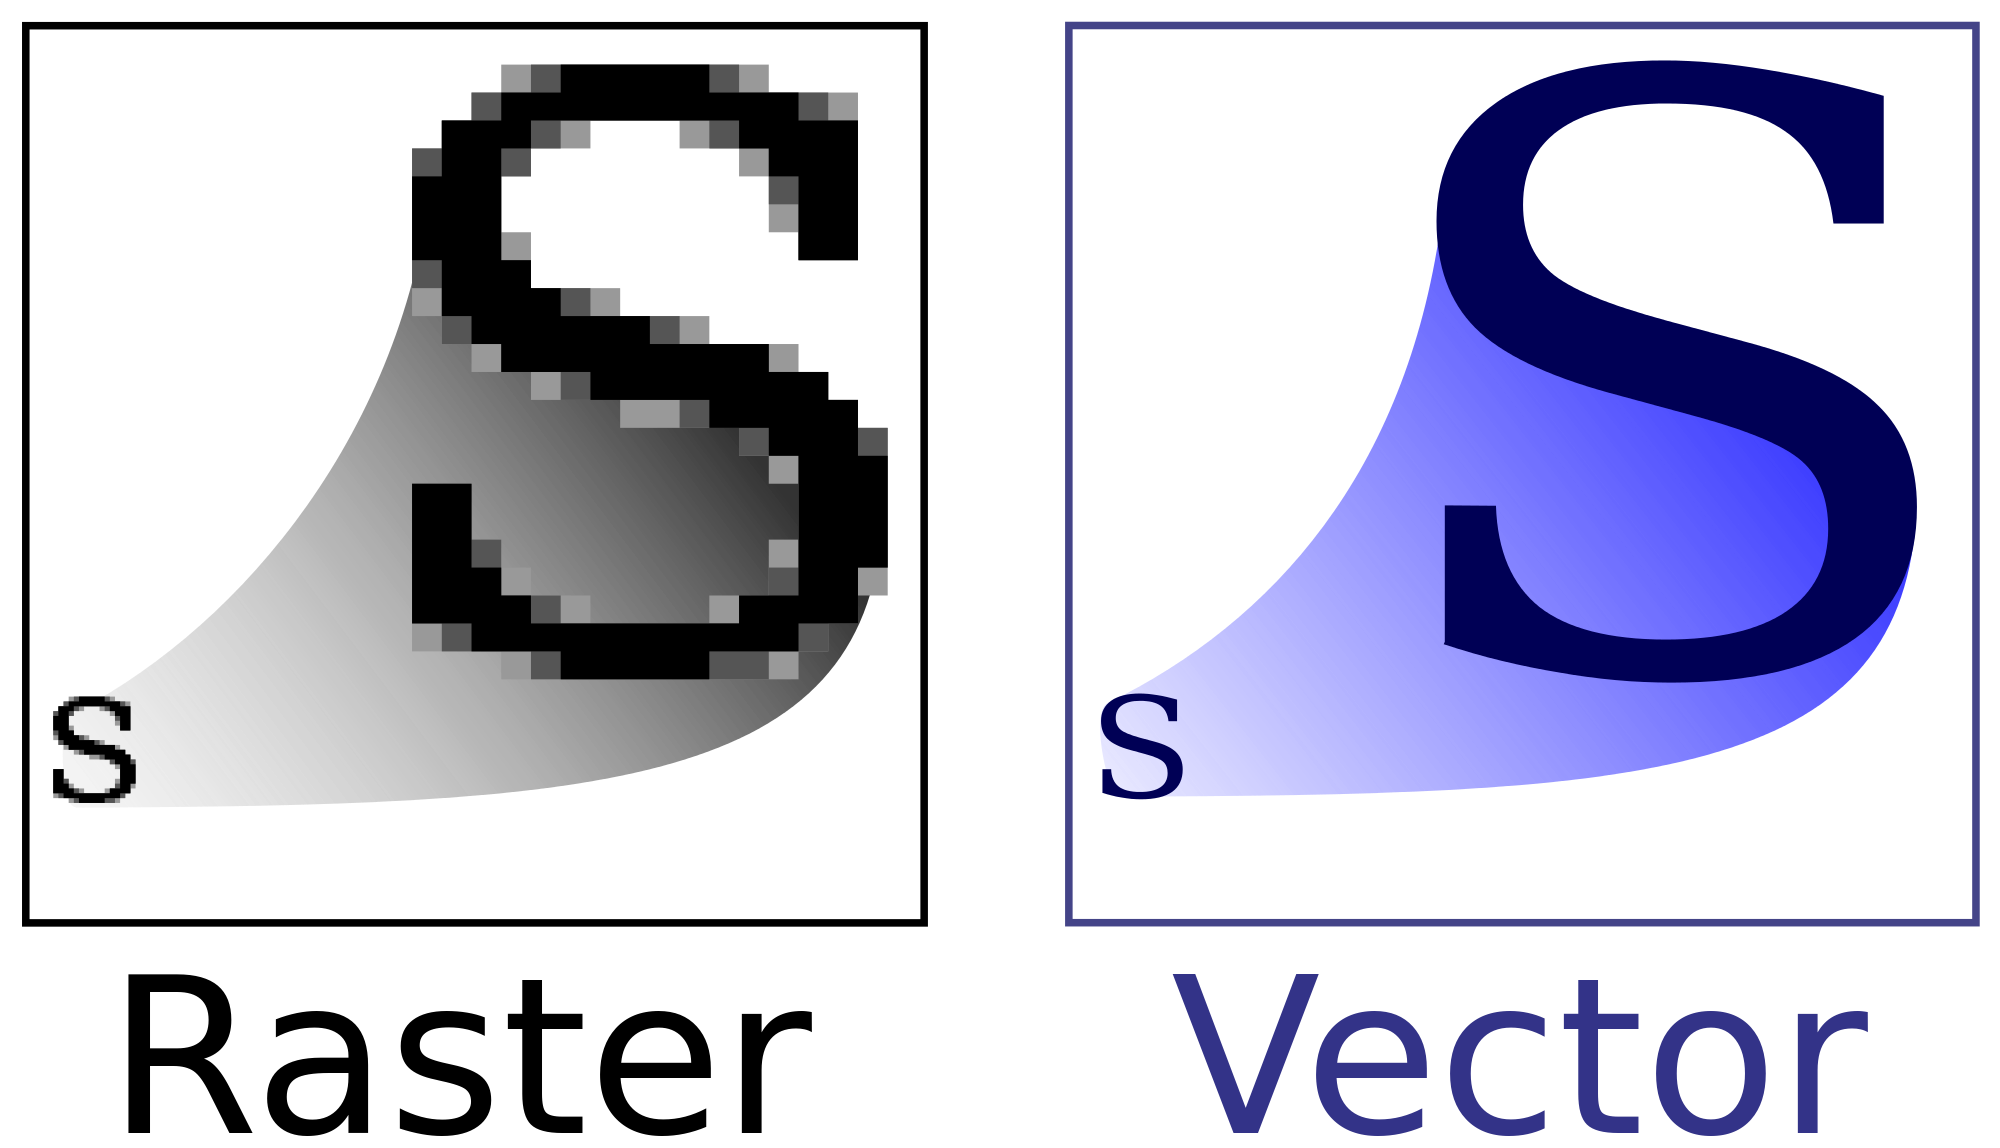
\includegraphics[width=0.5\linewidth]{images/bm_vs_svg.png}
\caption{Scaling comparison between raster graphics and vector graphics \cite{svg}.}
\label{fig:vectorscaling}
\end{figure}

Due to the geometrical nature of vectors, and the non-geometrical nature of the real world, it's not practical to use vector graphics to represent photographs.
Computer generated text, drawings or imagery, for use in graphical design, are the most common use case for vector graphics today, since the graphics can easily be scaled up or down by demand.
Most professional image processing and design software, e.g. Adobe Illustrator, support vector graphics.
At the time of writing, \texttt{svg} and \texttt{ai} are two examples of commonly used vector formats.

%In vector graphics an image is created by assembling a set of figures into a more complex image.
%These base figures are for example lines, circles, ellipses or curves. //TODO: Maybe reformat this

\subsubsection{Bézier curves}
\label{sec:bezier}
A popular type of curve in vector graphics is the Bézier curve.
Bézier curves can represent everything from a straight line to very complex paths with a lot of turns and changes in direction.
A Bézier curve is defined by a series of control points ranging from \(P_0\) to \(P_n\).
n is called the order of the curve and as such you end up with linear (n = 1), quadratic (n = 2), and cubic (n = 3) Bézier curves.
Formulas for Bézier curves with n=1,2,3 are shown in Equation \ref{equ:line} to \ref{equ:cube}.
B(t) is the point on the curve at t.
As t can be incremented as little or as much as wanted points on the curve can be calculated as granularly as desired.

\begin{cequation}[H]
	\begin{equation}
	    \label{equ:line}
		\mathbf{B}(t)=\mathbf{P}_0 + t(\mathbf{P}_1-\mathbf{P}_0)=(1-t)\mathbf{P}_0 + t\mathbf{P}_1 \mbox{ , } 0 \le t \le 1
	\end{equation}
	\caption{Linear Bézier curve}
\end{cequation}

\begin{cequation}[H]
	\begin{equation}
		\mathbf{B}(t) = (1 - t)^{2}\mathbf{P}_0 + 2(1 - t)t\mathbf{P}_1 + t^{2}\mathbf{P}_2 \mbox{ , } 0 \le t \le 1
	\end{equation}
	\caption{Quadratic Bézier curve}
\end{cequation}

\begin{cequation}[H]
	\begin{equation}
	    \label{equ:cube}
		\mathbf{B}(t)=(1-t)^3\mathbf{P}_0+3(1-t)^2t\mathbf{P}_1+3(1-t)t^2\mathbf{P}_2+t^3\mathbf{P}_3 \mbox{ , } 0 \le t \le 1
	\end{equation}
	\caption{Cubic Bézier curve}
\end{cequation}

\subsection{Vector graphics in modern computing}

Vector graphics is not in frequent use today as a display technology, however it is widely used to represent data internally in a computer.
Two examples of vector technology in use today are the SVG format and text in TrueType \cite{truetype}.

Apple Inc. \cite{apple} uses vector graphics in their drawing engine that is available to all iOS and OS X application developers.
This drawing engine is called Quartz 2D \cite{quartz2d} and is widely used in order to make resolution independent user interfaces.
